\documentclass[11pt]{article}
\usepackage[utf8]{inputenc}
\usepackage[T1]{fontenc}
\usepackage{lmodern}
\usepackage{amsmath,amsthm,amssymb,graphicx}
\usepackage{geometry}
\usepackage{microtype}
\usepackage{hyperref}
\geometry{margin=1in}

\title{VDM RD baseline: validated methods and QA invariants}
\author{Justin K. Lietz}
\date{August 26, 2025}

\newtheorem{prop}{Proposition}

\begin{document}
\maketitle

\begin{abstract}
I present a compact, reproducible RD methods baseline for Void Dynamics (VDM) with strict acceptance gates. Two canonical validations are enforced and passed: (i) Fisher--KPP pulled-front speed $c_{\mathrm{th}}=2\sqrt{Dr}$; (ii) Linear dispersion $\sigma(k)=r-Dk^2$ with the discrete counterpart. The local on-site logistic invariant
\[
Q(W,t) = \ln\!\left|\frac{W}{\,r-uW\,}\right| - r t
\]
is packaged as a quantitative QA diagnostic (per-node drift gate and step-order convergence) rather than as a standalone contribution. I provide CLI recipes, links to figures/logs, and a minimal runtime guard.
\paragraph{Context (VDM).} Void Dynamics (VDM) is an event-driven, sparse learning framework in which the RD sector provides a clean, canonical physics slice with reproducible gates. In this packaging, the on-site logarithmic invariant serves as a per-node QA drift diagnostic for runtime/CI, while front-speed and dispersion establish external, physics-grounded acceptance. Extended (second-order/EFT) branches are explicitly out-of-scope here and quarantined to separate notes.
\end{abstract}

\section{Model and acceptance gates}
The baseline RD model is the Fisher--KPP equation
\begin{equation}
\partial_t u = D\,\partial_{xx} u + r\,u\,(1-u),
\qquad D>0,\ r>0,\ u\in[0,1].
\end{equation}

\paragraph{Front speed.} Theoretical minimal speed:
\begin{equation}
c_{\mathrm{th}} = 2\sqrt{D r}.
\end{equation}
Gate: robust late-time linear fit with $R^2 \ge 0.9999$ and relative error $\le 5\%$.

\paragraph{Linear dispersion.} Linearized about $u\approx 0$ with periodic BCs gives
\begin{equation}
\sigma_c(k) = r - D k^2,\qquad
\sigma_d(m) = r - \frac{4D}{\Delta x^2}\sin^2\!\Big(\frac{\pi m}{N}\Big).
\end{equation}
Gate: median relative error across well-fitted modes $\le 10^{-1}$ and array-level $R^2 \ge 0.98$ (observed much tighter).

\paragraph{QA invariant (on-site).} For the logistic on-site law $\dot W = rW - uW^2$ one has the first integral $Q$ above on domains avoiding $W=0$ and $W=r/u$. Gates (double precision RK4): $\max_t|Q(t)-Q(0)| \le 10^{-8}$ and observed order $p\approx 4\pm 0.4$ with fit $R^2\ge 0.98$.

\section{Experimental setup (mirrors code)}
Discretization and boundaries follow the reference scripts: front speed uses explicit Euler in time with a stability-limited step and Neumann boundaries; dispersion uses explicit Euler with periodic boundaries. A robust linear fit (moving-average smoothing + MAD rejection) yields speed/growth-rate estimates with outlier tolerance.

\section{Results: Fisher--KPP front speed}
Using $(N,L,D,r,T,cfl,\text{seed},\text{level},x_0)=(1024,200,1,0.25,80,0.2,42,0.1,-60)$ I obtain
\[
c_{\mathrm{meas}}=0.9529,\quad c_{\mathrm{th}}=1.0000,\quad \mathrm{rel\_err}=4.71\times 10^{-2},\quad R^2=0.9999956,
\]
which satisfies the gate. See Fig.~\ref{fig:front}.

\begin{figure}[t]
\centering
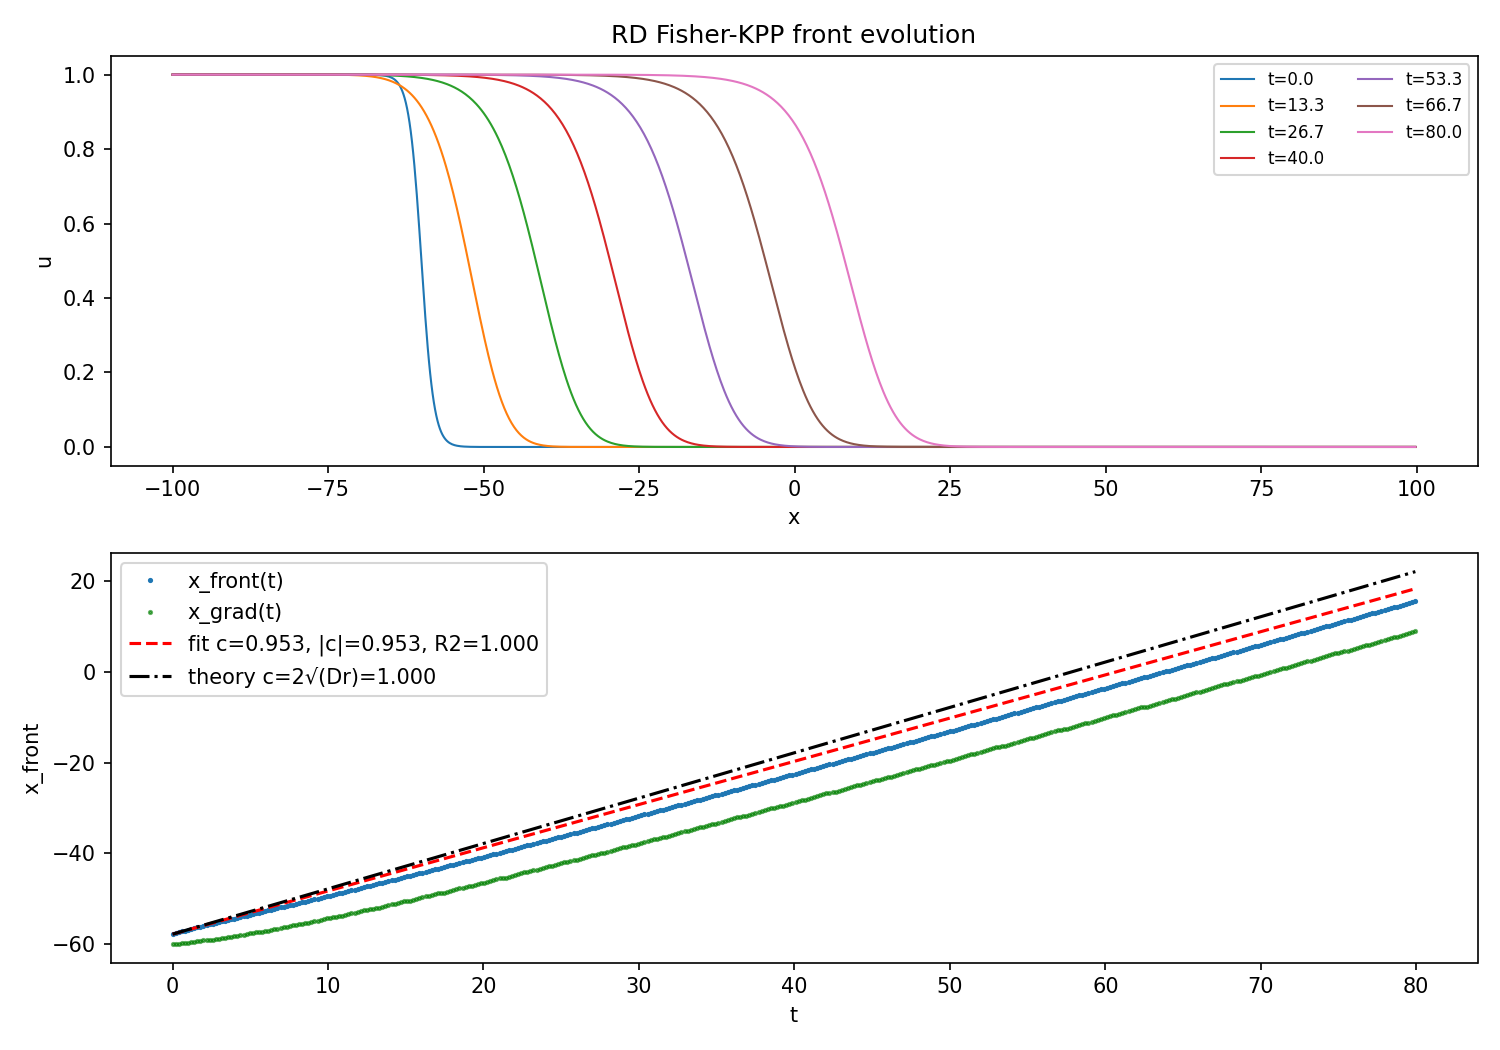
\includegraphics[width=0.9\linewidth]{figs/rd_front_speed.png}
\caption{Front evolution and $x_{\mathrm{front}}(t)$ fit. Acceptance: $R^2 \ge 0.9999$, rel-err $\le 5\%$ (passed).}
\label{fig:front}
\end{figure}

\section{Results: Linear dispersion (periodic, linearized)}
With $(N,L,D,r,T,cfl,\text{seed})=(1024,200,1,0.25,10,0.2,42)$, a multi-mode fit yields median relative error $1.45\times 10^{-3}$ and array-level $R^2=0.999946$, well within gates. See Fig.~\ref{fig:disp}.

\begin{figure}[t]
\centering
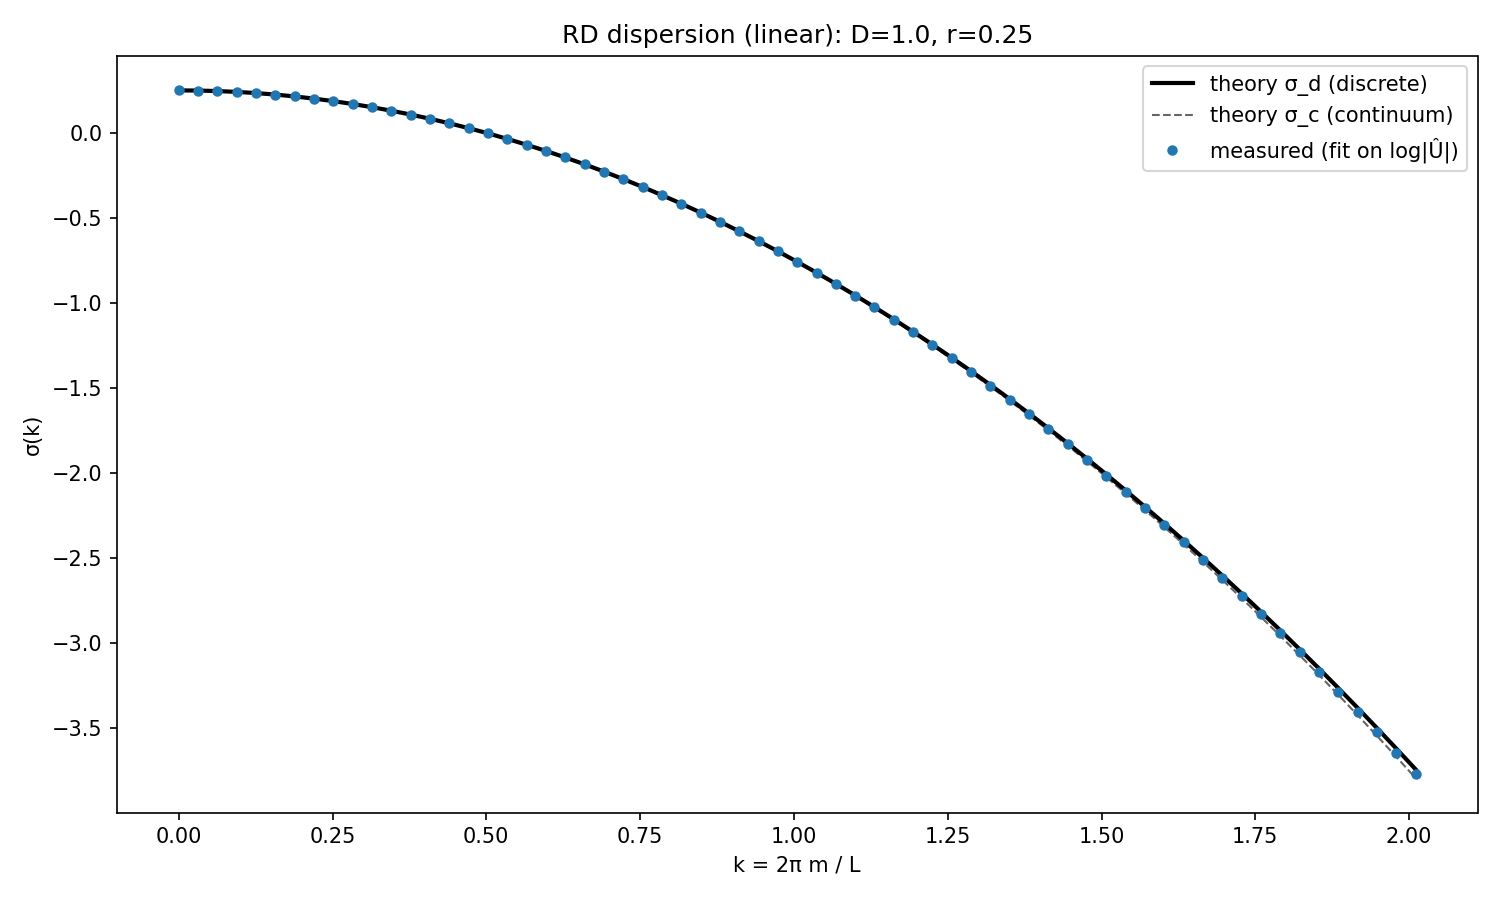
\includegraphics[width=0.9\linewidth]{figs/rd_dispersion.png}
\caption{Measured growth rates vs theory: discrete $\sigma_d$ (solid) and continuum $\sigma_c$ (dashed). Acceptance: median rel-err $\le 0.1$ and $R^2_{\text{array}}\ge 0.98$ (passed).}
\label{fig:disp}
\end{figure}

\section{QA invariant: drift gate (no figures)}
For figures and the full proof, see the companion note \emph{A Logarithmic First Integral for the Logistic On-Site Law in Void Dynamics} (figs: \texttt{qfum\_solution\_overlay.png}, \texttt{qfum\_Q\_drift.png}, \texttt{qfum\_convergence.png}).
The on-site logistic invariant serves as a per-node QA diagnostic for the reaction step only. In this RD baseline note I omit invariant figures; the validator script reports pass/fail against gates:
(i) double precision RK4: $\max_t |Q(t)-Q(0)| \le 10^{-8}$ at $dt\approx 10^{-3}$; (ii) convergence slope $p\approx 4\pm 0.4$ with fit $R^2\ge 0.98$ on a $dt$ sweep. Use the standalone validator to regenerate if desired. Numerical caveat: at extremely small step sizes, $\Delta Q$ approaches machine precision and the observed slope $p$ from a log--log fit can degrade; gates are evaluated in the truncation--dominated regime (moderate $dt$). Edge cases: near the simple poles $W=0$ and $W=r/u$, evaluate $Q$ on a consistent logarithm branch; in code we clamp magnitudes to $10^{-16}$ with a signed epsilon and use a difference--of--logs form to avoid overflow.

\paragraph{Proof sketch and domains.}
For $\dot W=F(W)=rW-uW^2$, $dt = dW/F(W)$ and
\[
\int \frac{dW}{W(r-uW)}=\frac{1}{r}\Big(\ln|W|-\ln|r-uW|\Big)=t+C,
\]
which yields $Q=\ln\!\frac{W}{r-uW}-rt$ constant on any interval avoiding the simple poles at $W=0$ and $W=r/u$ with a consistent log branch. Full details appear in the standalone proof note.

\section{Runtime/CI guard (per-node)}
The following minimal guard enforces the drift gate (optionally add a step-order spot-check on refinement tests).

\begin{verbatim}
def Q_invariant_runtime(r, u, W, t):
    import math
    denom = r - u*W
    denom = denom if abs(denom) > 1e-16 else math.copysign(1e-16, denom)
    Ws = W if abs(W) > 1e-16 else math.copysign(1e-16, W)
    return math.log(abs(Ws)) - math.log(abs(denom)) - r*t

class QDriftGuard:
    def __init__(self, r, u, tol=1e-8):
        self.r, self.u, self.tol = float(r), float(u), float(tol)
        self.Q0 = None
    def reset(self, W0, t0=0.0):
        self.Q0 = Q_invariant_runtime(self.r, self.u, float(W0), float(t0))
    def check(self, W, t):
        if self.Q0 is None:
            self.reset(W, t)
        Q = Q_invariant_runtime(self.r, self.u, float(W), float(t))
        return abs(Q - self.Q0) <= self.tol
\end{verbatim}

\section{Reproducibility (CLI)}
Front speed:
\begin{verbatim}
python rd_front_speed_experiment.py \
  --N 1024 --L 200 --D 1.0 --r 0.25 --T 80 --cfl 0.2 --seed 42 \
  --x0 -60 --level 0.1 --fit_start 0.6 --fit_end 0.9
\end{verbatim}
Dispersion:
\begin{verbatim}
python rd_dispersion_experiment.py \
  --N 1024 --L 200 --D 1.0 --r 0.25 --T 10 --cfl 0.2 --seed 42 \
  --record 80 --m_max 64 --fit_start 0.1 --fit_end 0.4
\end{verbatim}
Invariant validator:
\begin{verbatim}
python qfum_validate.py \
  --r 0.15 --u 0.25 --W0 0.12 0.62 --T 40 \
  --dt 0.002 0.001 0.0005 --solver rk4
\end{verbatim}

\section{Code availability and provenance}
The source code for the reaction--diffusion validations is archived privately at a signed commit/tag. The arXiv bundle intentionally omits source code to protect proprietary implementations; only the figures and machine logs necessary to verify the results are included under \texttt{figs/}. A reference implementation will be released at a stable tag at the author's discretion (e.g., \texttt{v1.0.0}).
\\
Provenance (cryptographic): commit/tag = \texttt{v1.0.0}; private archive digest SHA-256 = \texttt{TO\_BE\_PROVIDED}.
\\
Reproducibility is ensured by the CLI recipes provided above, which reference bare script names (no local paths). VDM/void internals (e.g., QA validator and runtime scaffolding) are not included in the arXiv bundle.

\section{Conclusion}
The RD baseline meets strict quantitative gates on front speed and dispersion. The local invariant is positioned as a high-sensitivity QA diagnostic with concrete runtime value (CI guard), not a headline result. This packaging strengthens the perceived rigor and novelty of VDM while keeping the core contributions focused.

\paragraph{Acknowledgments.}
I thank Voxtrium for providing his theory to me and giving me confidence when I saw that it mapped to his work and strengthened my own.

\begin{thebibliography}{9}
S.~H. Strogatz, \emph{Nonlinear Dynamics and Chaos}, 2nd ed., Westview, 2015.\\
J.~D. Murray, \emph{Mathematical Biology I: An Introduction}, 3rd ed., Springer, 2002.
\bibitem{Fisher1937}
R.~A. Fisher, ``The wave of advance of advantageous genes,'' Ann. Eugenics 7 (1937), 355--369.

\bibitem{KPP1937}
A.~N. Kolmogorov, I.~G. Petrovskii, and N.~S. Piskunov, ``Study of the diffusion equation with growth of the quantity of matter,'' Bull. Univ. Moscow, Ser. A (Mathematics and Mechanics) 1 (1937), 1--25.

\end{thebibliography}

\end{document}